
\chapter{Sub-ADC Design}
\graphicspath{{Sub-ADC Design/Vector/}{Sub-ADC Design/}}

Figure 3.1 shows the common ADC 
topologies used in these serial links, 
which include flash, binary/multibit 
search, and successive approximation 
register (SAR). Flash ADCs employ 
comparators at each reference level, 
with a 6-b flash ADC requiring 63 comparators that simultaneously evaluate 
over a single cycle. This allows for very 
high-speed operation with relatively 
low time-interleave factors between 
four and eight. The main downside is the large comparator count, although 
rectifying architectures can reduce 
this. Overall, flash ADCs are a reasonable choice for PAM2, but the resolution is a bit low for PAM4.\\

\begin{figure*}
	\centering
	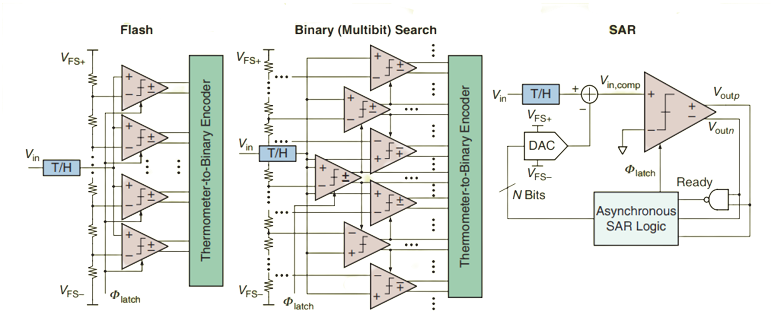
\includegraphics[width=12cm,height=6cm]{fig3_1.png}
	\caption{The common ADC topologies used in serial link receivers. [7]}
	\label{adc_topo}
\end{figure*}

Binary or multi-bit search ADCs 
combine desirable properties of flash 
and SAR ADCs. While conventional 
binary search ADCs have the same 
number of comparators as a flash 
ADC, the architecture employs a binary search algorithm with the most 
significant bit (MSB) comparator's output deciding which MSB-1 comparator is clocked, and so on. This results 
in only the necessary comparators 
evaluating, or six in a 6-b converter. 
The binary search ADC avoids the digital-to-analog converter (DAC) settling 
and logic delay present in SARs but is 
slower than a flash due to the serial 
comparator evaluation. Overall, this 
is also a good choice for PAM-2 applications, but the area is often high for 
PAM-4 applications.\\
An SAR ADC employs a binary search 
conversion over multiple clock cycles. 
The simplest implementations require 
only one comparator per unit ADC, 
whose decision adjusts a reference DAC 
to make the full signal quantization in a 
successive approximation manner, with 
a 6-b converter clocking the comparator 
six times. This results in a slower unit 
ADC relative to flash or binary search, 
with high-speed converters using higher 
interleave factors of 32–128. 
This is an excellent choice for 6–8-b resolution to support both PAM-2 and PAM-4, 
and it is the dominant architecture for 
PAM-4 ADC-based receivers. Given this, 
the next section provides an overview of key ADC circuits in the context of a time-interleaved SAR ADC. Note that many of 
the circuit concepts are also relevant to 
other ADC topologies.

\begin{figure*}[h]
	\centering
	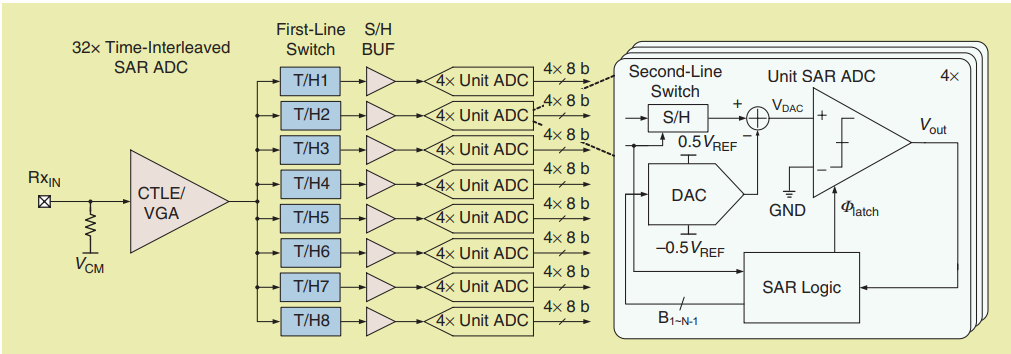
\includegraphics[width=10cm,height=6cm]{fig3_2.png}
	\caption{A 32-way time-interleaved SAR ADC. GND: ground; S/H BUF: sample/hold buffer. [7]}
	\label{TI-ADC}
\end{figure*}

%%%%%%%%%%%%%%%%%
%%%%%%%%%%%%%%%%%%
%%%%%% Chapter 3 Section 1
%%%%%%%%%%%%%%%%%
%%%%%%%%%%%%%%%%%%
\section{Sampling Switch}

The input T/H circuit must track 
and sample/hold the full-bandwidth 
input signal for further sampling by 
the unit ADCs. Due to this high-bandwidth requirement, many high-speed 
ADCs employ a bootstrapped T/H 
switch [11]. The collection of transistors and the offset storage capacitor 
shown in Figure 5 produce a signal independent overdrive on the main 
sampling switch to keep the tracking bandwidth constant. When the 
clock is low and the switch is off, the 
capacitor is precharged to VDD. One 
terminal of the capacitor is then connected to the input when the clock 
goes high, forcing the other terminal 
to VDD above it, which should result 
in a signal-independent VDD overdrive on the switch when it is on. This 
results in an improvement in signal-to-noise-and-distortion ratio (SNDR), 
particularly at high frequencies.

\begin{figure*}[h]
	\centering
	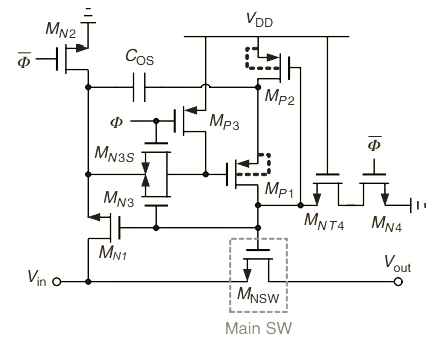
\includegraphics[width=10cm,height=7cm]{fig3_3.png}
	\caption{Bootstrapped T/H [7]}
	\label{TI-ADC}
\end{figure*}

After the second-line switch, the 
unit ADC consists of the capacitive 
reference DAC, the comparator, and 
SAR logic. The DAC generates residue 
signals for each bit conversion by 
subtracting a binary weighted reference from the sampled input signal. 
This is done via charge sharing in a 
capacitive DAC, with a typical $65\,nm$ 
CMOS implementation.



\section{StrongARM Latch}
\rhead{StrongARM Latch}
\label{StrongARM Latch}


The comparator is a sense amplifier that is desgined by using a StrongARM Latch topology. The StrongARM latch topology finds 
wide usage as a sense amplifier, 
a comparator, or simply a robust 
latch with high sensitivity. The term 
“StrongARM” commemorates the use 
of this circuit in Digital Equipment 
Corporation’s StrongARM microprocessor, but the basic structure was 
originally introduced by Toshiba’s 
Kobayashi. The StrongARM 
latch has become popular for three 
reasons: 
\begin{enumerate}[1.]
	\item it consumes zero static power
	\item it directly produces rail-to-rail outputs
	\item its input-referred offset arises from primarily one differential pair.
\end{enumerate}

\begin{figure*}[h]
	\centering
	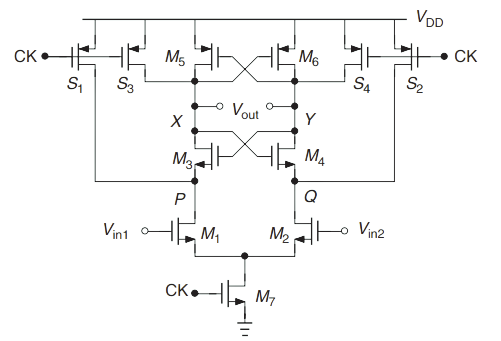
\includegraphics[width=10cm,height=6cm]{fig3_4.png}
	\caption{Modified StrongARM Latch [7]}
	\label{SAL}
\end{figure*}

The comparator makes a decision 
on the DAC signal to generate the output bits that serve as the binary search 
codes for the SAR logic that controls 
the DAC. Noise 
and offset considerations generally set 
the minimum comparator size. However, the brute-force design of a comparator for a given offset performance 
leads to excessive power and area in 
modern CMOS processes.

\newpage
\section{SAR Logic}
\rhead{SAR Logic}

Finally, the SAR logic generates both 
the comparator clock and the DAC control signals based on the comparator 
output. A conventional synchronous 
SAR ADC uses logic that generates an 
internal clock operating at N + 1 times 
the unit ADC sampling frequency to 
allow for one tracking cycle and N-bit 
conversion cycles. However, given 
metastability considerations, each cycle should be timed to satisfy the worst-case comparator input that will occur 
only once in the multi-bit conversion.